\documentclass[journal]{IEEEtran}

% Core packages
\usepackage{cite}
\usepackage{amsmath,amssymb}
\usepackage{graphicx}
\usepackage{booktabs}
\usepackage{multirow}
\usepackage{float}
\usepackage{placeins}
\usepackage{flafter} % a float never appears before its first reference
\usepackage{dblfloatfix}
\usepackage{xcolor}
\usepackage{url}
\usepackage[hidelinks]{hyperref}
\usepackage[T1]{fontenc}
\usepackage[utf8]{inputenc}

\graphicspath{{./images/}}

% Float placement tuning for IEEE two-column layout
\renewcommand{\dbltopfraction}{0.95}
\renewcommand{\topfraction}{0.95}
\renewcommand{\textfraction}{0.05}
\renewcommand{\floatpagefraction}{0.80}
\renewcommand{\dblfloatpagefraction}{0.80}
\setcounter{topnumber}{5}
\setcounter{dbltopnumber}{5}
\setcounter{totalnumber}{8}

\usepackage{etoolbox}

\makeatletter
\patchcmd{\thebibliography}
  {\clubpenalty4000}
  {\clubpenalty4000
   \setlength{\itemsep}{0pt}
   \setlength{\parskip}{0pt}}
  {}{}
\makeatother


\begin{document}
\title{ADMET-Bench: Task-Dependent Performance of GNNs and Pretrained Models in ADMET Prediction}

\author{
\IEEEauthorblockN{
Martin Stamenov\IEEEauthorrefmark{1},
Mila Gjurovska\IEEEauthorrefmark{1},
Viktorija Vodilovska\IEEEauthorrefmark{2} and
Ilinka Ivanoska\IEEEauthorrefmark{1}
}

\IEEEauthorblockA{\IEEEauthorrefmark{1} %1st affiliation
Faculty of Computer Science and Engineering, Ss Cyril and Methodius University, Skopje, N. Macedonia}

\IEEEauthorblockA{\IEEEauthorrefmark{2} %2nd affiliation
Graduate School of Life Sciences, Utrecht University, Utrecht, The Netherlands}

martin.stamenov@students.finki.ukim.mk, mila.gjurovska@students.finki.ukim.mk, v.vodilovska@students.uu.nl, ilinka.ivanoska@finki.ukim.mk

\thanks{Ilinka Ivanoska is the corresponding author.}
\thanks{Martin Stamenov and Mila Gjurovska contributed equally.}
\thanks{Supported by Faculty of Computer Science and Engineering, Skopje, N. Macedonia.}
}

\maketitle

\begin{abstract}
The reliability of structure-based prediction of absorption, distribution, metabolism, excretion, and toxicity (ADMET) properties varies substantially across endpoints, yet many studies evaluate molecular models without accounting for endpoint difficulty. This work investigates the task-dependent performance of graph neural networks (GNNs), frozen pretrained molecular representations, and fingerprint-based baselines under scaffold-split evaluation, which better reflects generalization to novel chemical series. Using a unified experimental pipeline, we compare five model families across six Therapeutics Data Commons benchmarks covering four pharmacokinetic regression tasks and two toxicity classification tasks, and evaluate seven hyperparameter optimization (HPO) algorithms under a fixed 50-trial budget. Results reveal substantial differences in endpoint learnability. For structure-driven tasks such as hERG toxicity and Caco-2 permeability, GNNs achieve the strongest performance (hERG AUC $=$ 0.825 best HPO trial, $0.796$ multi-seed median). For the moderately structure-driven Tox21 NR-AR benchmark, GNNs also perform best (AUC $=$ 0.742 best HPO trial, $0.710$ multi-seed median). In contrast, for pharmacokinetic endpoints including hepatocyte clearance and half-life, all evaluated models produce near-zero or negative predictive accuracy, suggesting that molecular structure alone provides limited predictive signal. Across datasets, no HPO method consistently outperforms random search at a 50-trial budget. These findings indicate that ADMET prediction should be treated as an endpoint-specific problem rather than a single modeling task and highlight the importance of scaffold-based evaluation for realistic assessment of molecular machine-learning models.
\end{abstract}

\begin{IEEEkeywords}
graph neural networks, ADMET prediction, molecular property prediction, scaffold-split, pretrained models, drug discovery, benchmarking
\end{IEEEkeywords}


\section{Introduction}
\label{sec:intro}

\IEEEPARstart{P}{redicting} molecular ADMET (Absorption, Distribution, Metabolism, Excretion, and Toxicity) properties is a central task in computational drug discovery, enabling early identification of promising candidates and flagging safety liabilities before costly synthesis and \emph{in vivo} testing~\cite{zhang2025admet}. Graph Neural Networks (GNNs) have become prominent in this domain by treating molecules as graphs in which atoms serve as nodes and bonds as edges, enabling task-specific learning through message passing that encodes both local chemical motifs and global topological patterns inaccessible to fixed-length descriptors~\cite{gilmer2017neural, yang2019dmpnn, attentiveFP}.

Beyond GNNs, a diverse range of approaches has been applied to ADMET prediction. Pretrained molecular encoders such as ChemBERTa~\cite{chemberta2} and MolCLR~\cite{molclr} leverage self-supervised learning on large molecular corpora to produce reusable representations. Classical fingerprint-based methods, including Morgan (ECFP) fingerprints~\cite{rogers2010ecfp} paired with traditional ML or MLP predictors, remain competitive baselines~\cite{maplight, rdkit2d_mlp}. Although these approaches differ in architecture and encoding strategy, all model families evaluated here rely exclusively on molecular structure as input, representing the same underlying 2D molecular graph or SMILES string~\cite{weininger1988smiles} through different feature representations. Across these paradigms, strong predictive performance has been reported, often achieving state-of-the-art results on individual tasks~\cite{huang2021therapeuticsdatacommonsmachine}.

Despite this progress, model selection in practice remains unclear. Different models perform inconsistently across tasks, and most published studies optimize performance for individual architectures or compare methods under different splits and experimental conditions, making direct comparison unreliable~\cite{wu2018moleculenet, yang2019dmpnn}. Crucially, many works rely on random data splits, which allow structurally similar molecules to appear in both training and test sets, producing overly optimistic estimates that do not reflect the real-world scenario of predicting properties for new chemical scaffolds. As a result, practitioners still lack consistent guidance on model selection, endpoint-specific reliability, and the conditions under which molecular structure alone provides sufficient predictive information~\cite{wu2018moleculenet, huang2021therapeuticsdatacommonsmachine}.

Scaffold-based splitting~\cite{doi:10.1021/jm9602928} partitions compounds by core ring structures and serves as a realistic evaluation protocol reflecting prospective drug discovery, where models must generalize to novel chemical series. In this work, we investigate how predictive performance depends on the underlying task and evaluation protocol, with a focus on identifying when molecular structure alone provides sufficient signal. This issue is particularly important for pharmacokinetic endpoints such as clearance and half-life, where inaccurate predictions can affect compound prioritization. Models that appear accurate under weak evaluation protocols may provide misleading support for early-stage screening decisions.

Benchmarking should therefore identify not only which model performs best, but also which endpoints are predictable from molecular structure under realistic scaffold-shift conditions. This motivates endpoint-specific model selection, where the modeling approach is chosen according to the biological and experimental characteristics of the endpoint. From a biomedical informatics perspective, ADMET predictors act as decision-support components in early-stage drug-discovery pipelines. If such models are evaluated under overly optimistic protocols, they may produce overconfident predictions for novel scaffolds and misguide prioritization. Understanding endpoint-specific reliability under scaffold shift is therefore essential for trustworthy AI in translational drug-discovery workflows.

The main contributions of this study are as follows:
\begin{itemize}
 \item A systematic benchmark of graph-based, fingerprint-based, and pretrained molecular representation models across six ADMET endpoints from the TDC benchmark.
 \item Evaluation under scaffold-split conditions, enabling realistic assessment of generalization to structurally distinct compounds.
 \item Analysis of model behavior across endpoints with different biological characteristics, showing how predictive performance varies between permeability, toxicity, clearance, and half-life tasks.
 \item Assessment of seven hyperparameter optimization strategies and whether optimization consistently improves performance across model families and endpoints.
 \item Identification of endpoint-specific cases where molecular structure provides sufficient predictive signal, and cases where structure-only representations remain limited, motivating biological or assay-level information in future ADMET models.
\end{itemize}

The remainder of this paper is organized as follows. Section~II reviews related work. Section~III describes materials and methods. Section~IV presents experimental results. Section~V discusses implications and limitations. Section~VI concludes.

\section{Related Work}
\label{sec:related}

\subsection{ADMET Prediction}

The TDC ADMET benchmark~\cite{huang2021therapeuticsdatacommonsmachine} has become the standard evaluation platform for molecular property prediction. Representative molecular-property prediction approaches include fingerprint-based methods such as MapLight and RDKit2D+MLP, graph neural networks including GCN, GIN, D-MPNN and AttentiveFP, and pretrained molecular foundation models such as MolCLR and ChemBERTa. These approaches span fixed descriptors, task-specific graph learning, and self-supervised molecular representation learning.

The TDC leaderboards~\cite{tdc_admet_leaderboard} reveal that several top-performing approaches rely on comparatively simple architectures. MapLight~\cite{maplight} uses random forests and SVMs on node embeddings, while RDKit2D+MLP~\cite{rdkit2d_mlp} passes 200 physicochemical descriptors through a standard MLP. On certain datasets, even Random Forest or XGBoost achieves top results, motivating ensemble approaches such as FCA~\cite{cfa}.

Among GNN-based methods, AttentiveFP~\cite{attentiveFP} employs GCN/GAT layers with GRU-based attention readout, achieving top-5 results on many TDC datasets. Standard architectures appearing prominently in molecular benchmarks include GCN~\cite{kipf2017gcn}, GIN~\cite{xu2019gin}, and D-MPNN~\cite{yang2019dmpnn}, which operates on bond-level rather than atom-level messages.

Self-supervised pretraining has been adapted from NLP to molecular graphs via two main paradigms: attribute masking~\cite{attrMasking}, which reconstructs removed node or edge features, and contrastive learning~\cite{contrativeLearning}, which trains encoders to produce similar embeddings for augmented views of the same molecule. MolCLR~\cite{molclr} extends contrastive learning with three graph augmentation strategies (atom masking, bond deletion, subgraph removal), demonstrating improved downstream ADMET prediction. These techniques underpin most pretrained molecular representation models, which follow a common paradigm: self-supervised pretraining on large unlabeled corpora, optional multi-task supervised training, and task-specific fine-tuning. Representative examples include DeepMol~\cite{deepMol} and MolE~\cite{molE}. ChemBERTa~\cite{chemberta2} applies a RoBERTa transformer to SMILES strings pretrained on 77M molecules from ZINC-15~\cite{sterling2015zinc15}, while MolBERT~\cite{molbert} combines SMILES masked language modeling with auxiliary physicochemical objectives. A practical concern with pretrained models is their large parameter count. MiniMol~\cite{miniMol} addresses this using MPNN++ ($\sim$10M parameters) to achieve competitive TDC performance at lower computational cost.

\paragraph{Scaffold Split Challenges}
Transformer-based models frequently show severe generalization drops under scaffold splitting, with strong validation scores that collapse toward chance-level performance on held-out scaffolds~\cite{yang2019dmpnn,chemberta2}. Wu et al.\cite{wu2018moleculenet} introduced MoleculeNet with scaffold-splitting to reflect prospective drug discovery generalization; we revisit this collapse in Section\ref{sec:results}.

\subsection{Hyperparameter Optimization for Molecular ML}

HPO is a key performance driver in molecular ML, where small, noisy datasets amplify sensitivity to hyperparameter configuration. Bergstra and Bengio~\cite{bergstra2012random} established Random Search as a strong baseline, showing it outperforms grid search when only a subset of hyperparameters is influential. Bayesian methods such as TPE~\cite{bergstra2011tpe}, implemented in Optuna~\cite{akiba2019optuna}, improve sample efficiency by modeling the hyperparameter-performance relationship. Population-based metaheuristics, including PSO~\cite{kennedy1995pso}, GA~\cite{holland1975ga}, and ABC~\cite{karaboga2005abc}, provide broader exploration but may require larger budgets to converge. SA~\cite{saopt} offers a middle ground by accepting suboptimal moves early to escape local optima. Despite their widespread use in combinatorial optimization, systematic comparisons of these HPO strategies for molecular property prediction remain scarce, particularly under scaffold-split protocols, motivating our evaluation within a unified ADMET benchmark.

\subsection{Challenges in Molecular ML}

ADMET prediction remains challenging because many endpoints exhibit distribution shifts under scaffold splitting, limited dataset sizes, and class imbalance. These factors can substantially affect model rankings and generalization estimates, motivating the use of multi-seed evaluation and confidence-interval-based reporting throughout this study.


\section{Materials and Methods}
\label{sec:methods}

\subsection{Framework Overview}
\label{sec:framework}

To compare model families under realistic generalization conditions, we use a benchmarking framework (Fig.~\ref{fig:benchmark-framework}) that applies the same scaffold partitions, datasets, and metrics across the GNN and the frozen-pretrained/fingerprint pipelines. The framework coordinates dataset loading, scaffold-split partitioning, training, metric computation, multi-seed analysis, and HPO comparison against Random Search. Fixing splits and metrics across models reduces experimental confounds and enables direct comparison between model families~\cite{wu2018moleculenet}.

\begin{figure}[!t]
 \centering
 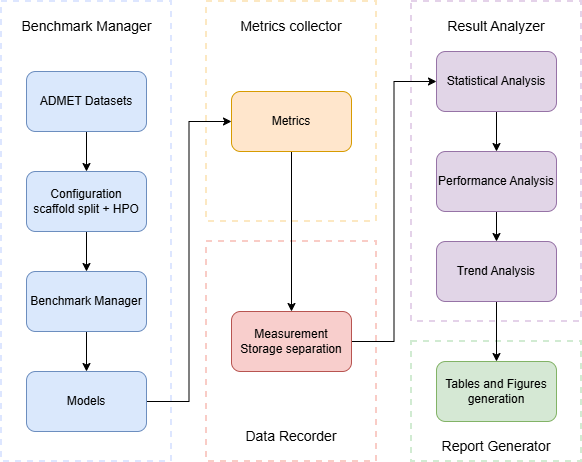
\includegraphics[width=\columnwidth,height=0.58\textheight,keepaspectratio]{architecture.png}
 \caption{Modular benchmarking architecture for evaluating molecular graph neural networks and pretrained models on ADME and toxicity prediction tasks. The framework consists of three layers: a benchmark orchestration layer coordinating datasets and experimental configurations, a model execution layer evaluating multiple neural architectures, and an evaluation pipeline.}
 \label{fig:benchmark-framework}
\end{figure}

\subsection{Datasets and Evaluation Protocol}
\label{sec:datasets}

We evaluate all models on six molecular property prediction tasks drawn from the TDC ADMET benchmark~\cite{huang2021therapeuticsdatacommonsmachine}, covering four pharmacokinetic (ADME) regression tasks and two toxicity classification tasks. This protocol reflects practical drug discovery scenarios, where models must generalize to novel chemical series. Fig.~\ref{fig:class-distribution} provides an overview of data provenance and class composition across all six datasets.

\subsubsection{ADME Regression Tasks}

\paragraph{Caco-2 Permeability (Caco2\_Wang)}
The dataset contains 910 compounds with permeability values reported in log(cm/s) units and is commonly used as an \emph{in vitro} surrogate of intestinal absorption~\cite{wang2016admet}.

\paragraph{Half-Life Prediction (Half\_Life\_Obach)}
The dataset contains 667 compounds with plasma half-life measurements. Target values are log-transformed prior to standardization to reduce skewness.

\begin{figure*}[!t]
 \centering
 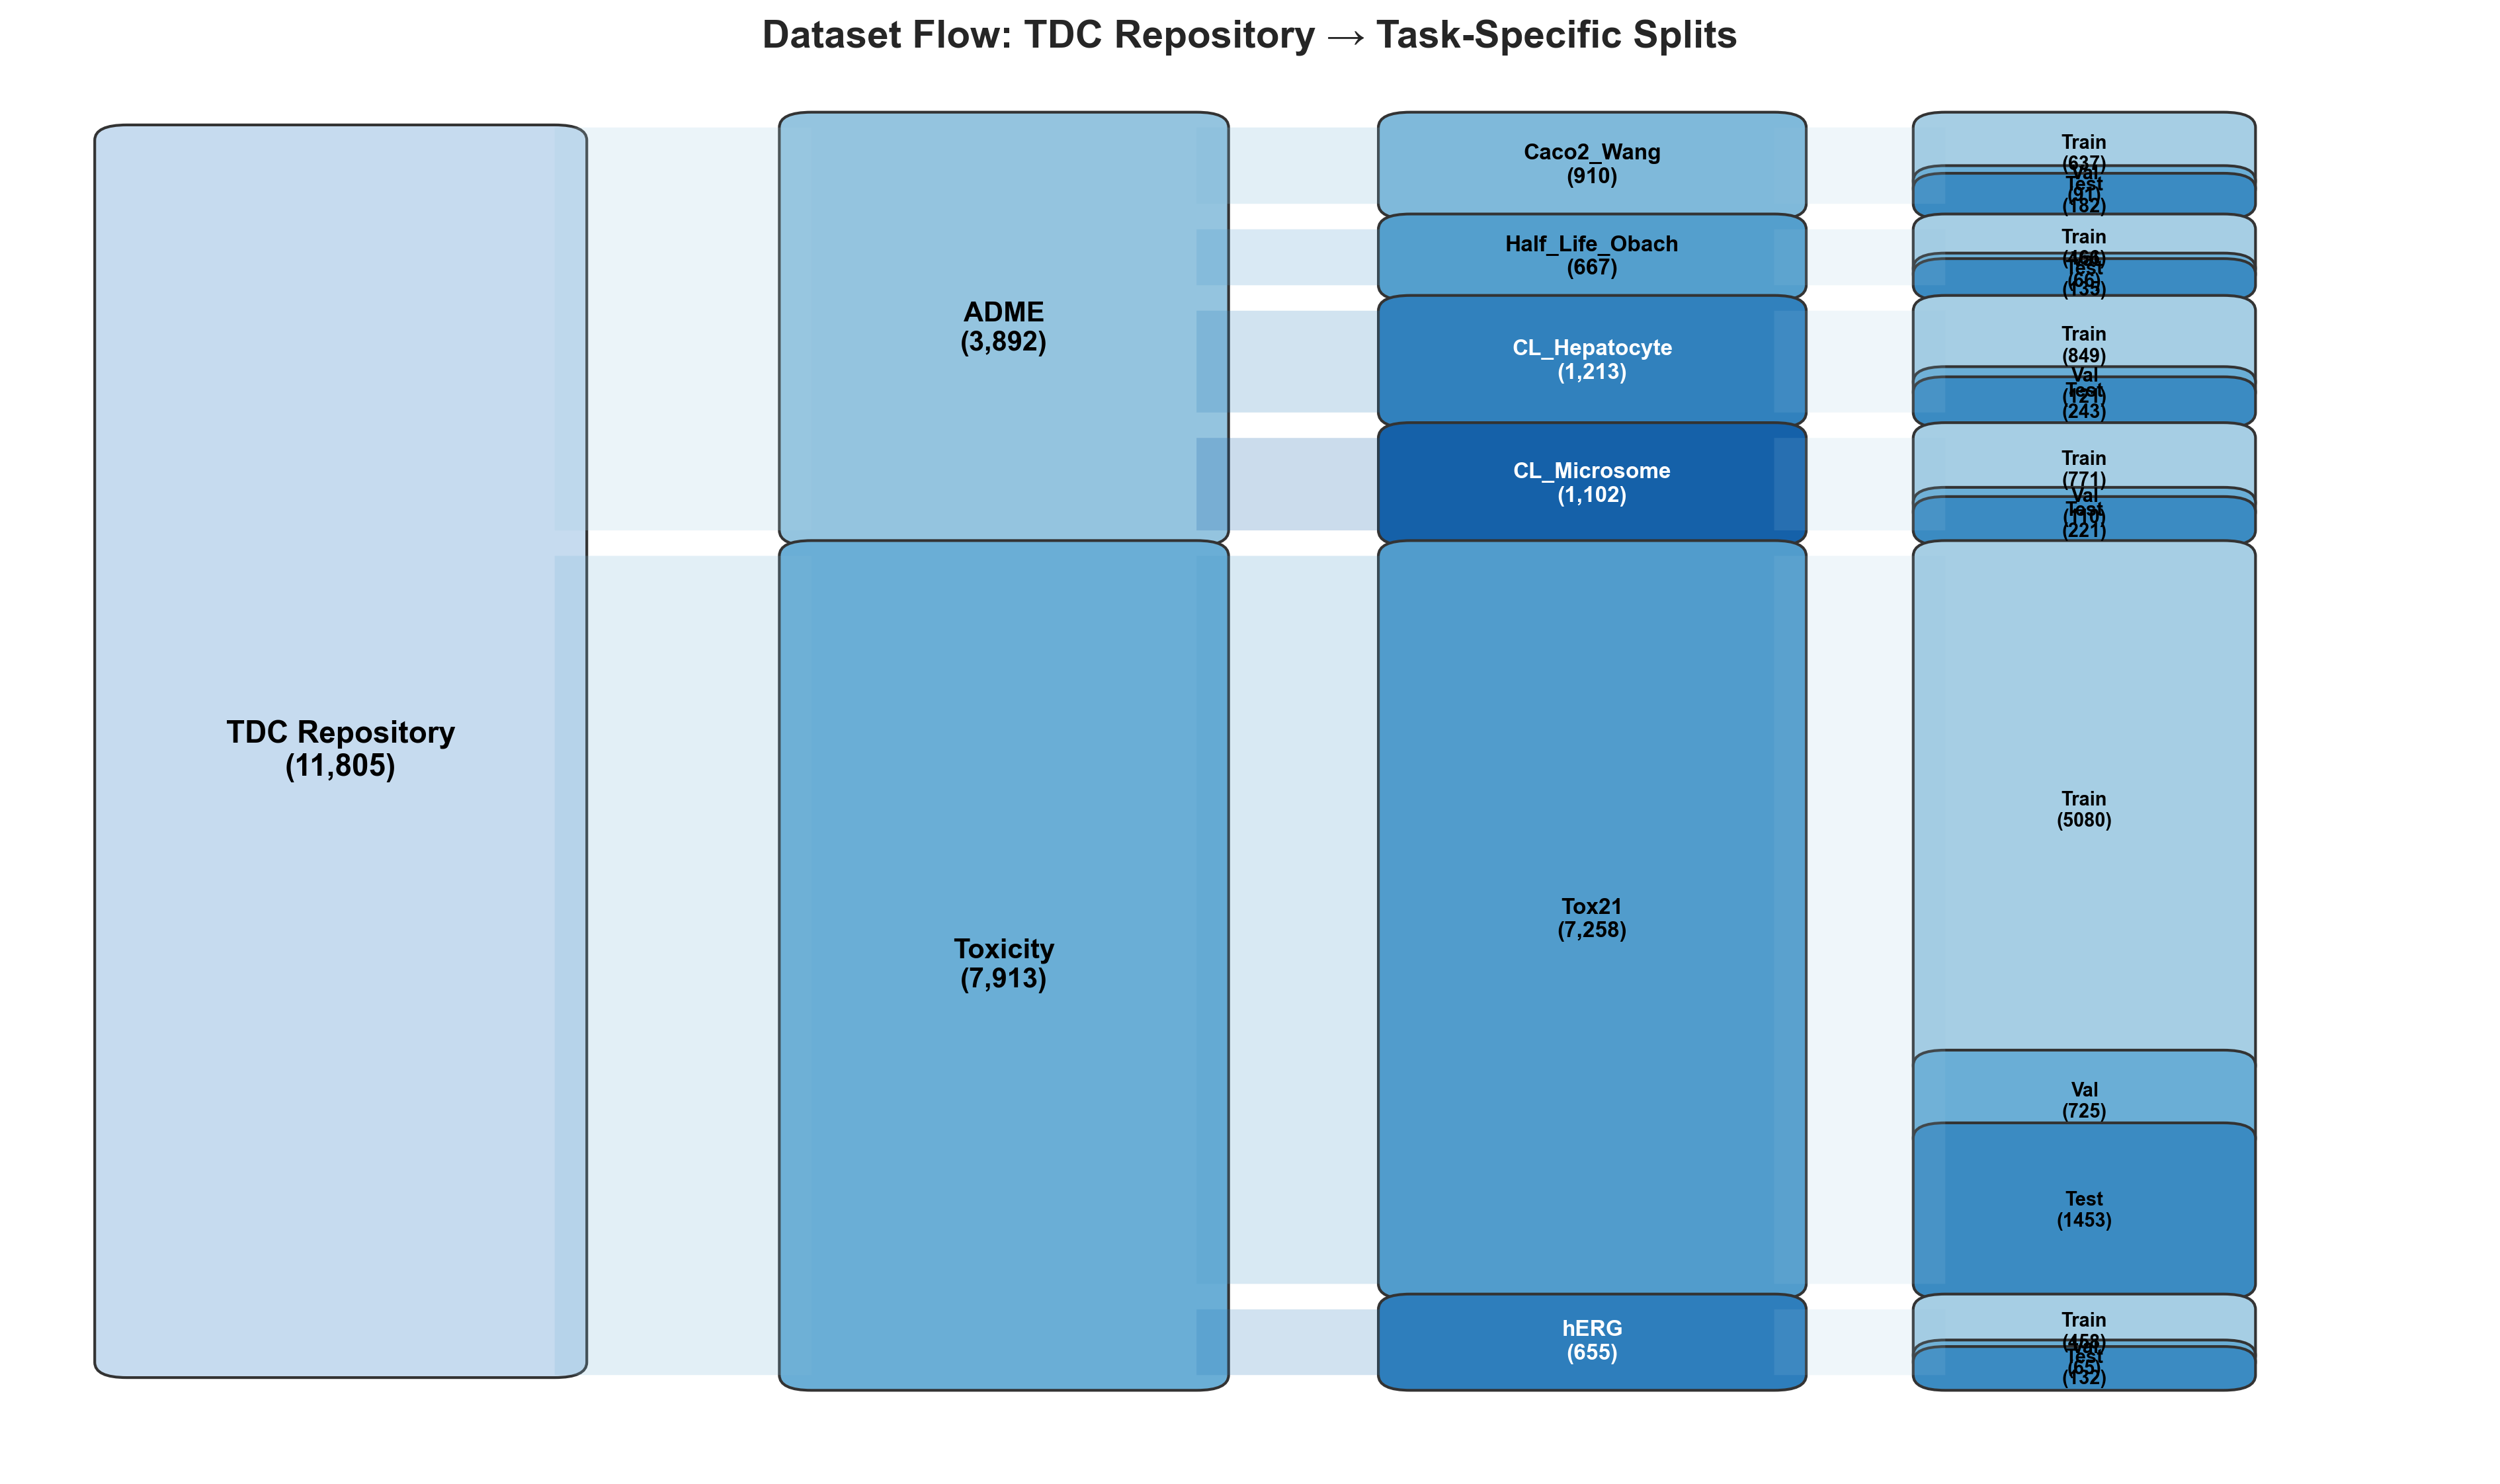
\includegraphics[width=0.75\textwidth,height=0.42\textheight,keepaspectratio]{sankey-diagram.png}
 \caption{Overview of data source and task labels. This flowchart details the $11{,}805$ total instances catalogued in the TDC Repository. After removing molecules with invalid SMILES or failed graph conversion, $10{,}627$ molecules are retained for training and evaluation.}
 \label{fig:class-distribution}
\end{figure*}

\paragraph{Hepatocyte Clearance (Clearance\_Hepatocyte\_AZ)}
The AstraZeneca dataset contains 1,213 compounds with intrinsic clearance measurements obtained from human hepatocyte assays~\cite{huang2021therapeuticsdatacommonsmachine}.

\paragraph{Microsomal Clearance (Clearance\_Microsome\_AZ)}
The AstraZeneca microsomal clearance dataset contains 1,102 compounds with human liver microsome measurements. Targets are log-transformed and standardized using training-set statistics.

\subsubsection{Toxicity Classification Tasks}

\paragraph{Tox21 Nuclear Receptor: Androgen Receptor (Tox21 NR-AR)}
The dataset contains 7,258 compounds with binary androgen receptor activity labels and exhibits substantial class imbalance, with approximately 4.2\% positive samples in the full corpus (rising to $\approx$4.9\% on the scaffold-split test set, see Section~\ref{sec:results}).

\paragraph{hERG Cardiotoxicity (hERG)}
The hERG dataset contains 655 compounds with blocker/non-blocker labels and is widely used for cardiotoxicity assessment~\cite{sanguinetti2006herg}.

\paragraph{Splitting and evaluation protocol}
We use the TDC scaffold-split function, which partitions compounds by Bemis-Murcko scaffolds~\cite{doi:10.1021/jm9602928} so that molecules with structurally distinct core rings appear in different folds. This approximates prospective deployment conditions, where a model must generalize to structurally distinct compound families not seen during training. We further subdivide the train set 90/10 (train/validation) using a fixed random seed (42) to enable early stopping and model selection without touching the held-out test set. The final split proportions are approximately 70/8/22 (train/validation/test) across all datasets, though because scaffold splitting assigns entire scaffold groups to the same partition, exact proportions may vary slightly.

During HPO, the test split remains \emph{fully held out}, model selection is performed solely on the validation metric. Final performance is reported once on the test split after HPO is complete, preventing any implicit information leakage from repeated test-set evaluations.

\paragraph{Target transformations}
For Half-Life, Hepatocyte, and Microsomal Clearance, targets are log-transformed using $y'=\log(\max(y,\epsilon))$, $\epsilon=10^{-3}$, followed by training-set z-score normalization. Caco-2 targets require only normalization, while classification labels remain binary.

\subsection{Model Families}
\label{sec:model_families}

We evaluate three distinct model paradigms under the same scaffold splits and evaluation metrics, allowing us to assess whether task-specific learning provides advantages over frozen pretrained representations and fixed fingerprint baselines.

\paragraph{GNN models}
We employ graph neural networks trained end-to-end on each task. The GNN backbone is based on stacked GraphConv layers~\cite{morris2019wlgnn} with batch normalization, ReLU activation, and additive residual connections, selected through a preliminary architecture comparison across eight GNN variants (Section~\ref{sec:arch_selection}). Each molecule is represented as a molecular graph constructed from SMILES using RDKit. Atom features include standard atom-level chemical descriptors (8 features); no bond features are used. The GNN encoder produces node embeddings aggregated into a graph-level representation using concatenated global mean and max pooling. Before the prediction head, this pooled representation is concatenated with a small vector of structure-derived physicochemical descriptors computed with RDKit (15 for the ADME/toxicity tasks, e.g.\ molecular weight, cLogP, TPSA, hydrogen-bond donors/acceptors, and Lipinski flags; a 7-descriptor subset for Caco-2). These descriptors carry no biological or assay information and are provided only to the GNN, not to the pretrained or fingerprint baselines. The combined representation is passed to an MLP prediction head with batch normalization and optional dropout; for the small Caco-2 dataset the GNN additionally applies dropout ($0.5$) and Gaussian target-label noise ($\sigma=0.05$). GNN models undergo full hyperparameter optimization (Section~\ref{sec:model_training}).

\paragraph{Pretrained models}
We evaluate two pretrained molecular encoders representing the two major pretrained paradigms: ChemBERTa~\cite{chemberta2} (SMILES-based transformer) and MolCLR~\cite{molclr} (graph-based contrastive model), as representative rather than exhaustive examples. For pretrained encoders, we use a frozen encoder and trainable MLP head setting: embeddings are extracted once per molecule, and an MLP is trained on the train split with early stopping based on the validation split. This frozen-encoder protocol isolates the quality of pretrained representations from downstream optimization effects.

\paragraph{Fingerprint baselines}
We evaluate two fingerprint-based approaches: (i) Morgan fingerprints (ECFP)~\cite{rogers2010ecfp} with an MLP predictor, and (ii) MolE-style learned fingerprints (MolE-FP) with an MLP predictor. The MolE-FP baseline is implemented as Morgan fingerprints followed by a learned projection inspired by the MolE approach~\cite{molE}, rather than the original pretrained MolE encoder. All baselines use the same dataset splits and evaluation metrics as the GNN experiments.

\subsection{Model Training and Configuration}
\label{sec:model_training}

\paragraph{GNN Training}
All GNN models were trained using the Adam optimizer with a batch size of 32. During HPO, models were trained for a maximum of 50 epochs per trial with early stopping (patience = 12). Regression models used mean squared error (MSE) loss, while classification models used binary cross-entropy (BCE) loss with logits. Gradient clipping was applied with a maximum norm of 1.0. The hyperparameter search space is defined in Supplementary Materials (Table S6).

\paragraph{Optimization algorithms}
We evaluate seven HPO strategies: Random Search~\cite{bergstra2012random}, Particle Swarm Optimization (PSO)~\cite{kennedy1995pso}, Artificial Bee Colony (ABC)~\cite{karaboga2005abc}, Genetic Algorithm (GA)~\cite{holland1975ga}, Simulated Annealing (SA)~\cite{saopt}, Hill Climbing (HC)~\cite{russell2010aima}, and Tree-structured Parzen Estimator (TPE)~\cite{akiba2019optuna}. Population-based methods use population size 16. SA uses $T_0=1.0$ with exponential cooling ($\alpha=0.99$), while TPE uses Optuna defaults with median pruning. Search spaces are provided in Supplementary Table S6. Each algorithm is allocated 50 trials per dataset, giving 2{,}100 GNN training runs from the optimizer comparison alone (seven optimizers $\times$ six datasets $\times$ 50 trials). In addition, the study includes a preliminary architecture-selection screen (reported in the Supplementary Material) and 30 multi-seed validation runs for the final selected models.

\begin{table}[!t]
\centering
\caption{Dataset statistics and evaluation metrics (TDC ADMET). ``TDC'' shows compounds catalogued and ``Used'' shows those retained after filtering. RMSE is the primary per-dataset regression metric, the scale-invariant R$^2$ is additionally used for cross-model comparison in Table~\ref{tab:model_comparison}.}
\label{tab:dataset_stats}
\small
\begin{tabular}{lccccc}
\toprule
\textbf{Dataset} & \textbf{Type} & \textbf{TDC} & \textbf{Used} & \textbf{Split} & \textbf{Metric} \\
\midrule
Caco2\_Wang & Regr. & 910 & 819 & Scaffold & RMSE \\
Half\_Life & Regr. & 667 & 601 & Scaffold & RMSE \\
Clear.\_Hep. & Regr. & 1,213 & 1,092 & Scaffold & RMSE \\
Clear.\_Mic. & Regr. & 1,102 & 992 & Scaffold & RMSE \\
Tox21 (NR-AR) & Class. & 7,258 & 6,533 & Scaffold & AUC \\
hERG & Class. & 655 & 590 & Scaffold & AUC \\
\bottomrule
\end{tabular}
\end{table}

\subsection{Experimental Setup}
\label{sec:experimental_setup}

\paragraph{Datasets}
Table~\ref{tab:dataset_stats} summarizes the dataset characteristics across all six tasks.

\paragraph{Evaluation metrics}
Model performance is assessed using RMSE, R$^2$, and MAE for ADME regression tasks, and AUC-ROC and F1-score for toxicity classification tasks. AUC-ROC is the primary ranking metric for classification, F1 is reported in addition because it is more sensitive to the minority class under strong class imbalance, and it is the classification metric used in the paired optimizer comparison, which can be seen in the Supplementary Material (Table~S3; per-optimizer F1 values in Table~S4).

\paragraph{Multi-seed validation}
To quantify robustness, we retrain the best HPO-selected configuration per dataset across five seeds $[42, 123, 456, 789, 1011]$. For the primary performance metrics reported in Table~\ref{tab:multiseed}, we use the median and full min--max range across seeds because the selected configuration diverges on a minority of seeds for some endpoints, making the mean unrepresentative. These medians provide a more conservative estimate than the optimistic best-of-50-trials result. Secondary imbalance-aware toxicity metrics (PR-AUC, F1, MCC) are reported as mean $\pm$ standard deviation to characterize variability.

\paragraph{HPO algorithm comparison}
We compare each optimizer against the Random Search baseline using paired performance differences across the six datasets rather than null-hypothesis significance tests. For every dataset we compute the improvement with a normalized direction so that positive values favor the optimizer (for RMSE, $\text{Random}-\text{Algo}$, for F1, $\text{Algo}-\text{Random}$). Because the datasets differ by orders of magnitude in scale, we express each difference as a percentage of the Random-Search baseline before aggregating. For each optimizer we report the win/tie/loss count, the mean relative improvement, a 95\% confidence interval obtained from 10{,}000 percentile bootstrap resamples of the six paired differences, and the paired effect size $d_z$ (mean divided by the standard deviation of the differences). The paired unit is the dataset ($n=6$), and all comparisons use final held-out test performance obtained after HPO model selection on the validation split. With only six paired observations, null-hypothesis significance tests are underpowered, we therefore rely on bootstrap confidence intervals and the paired effect size, which together summarize both the magnitude and the consistency of any improvement over Random Search.

\paragraph{Implementation}
Experiments were implemented in Python using PyTorch, PyTorch Geometric, RDKit, PyTDC, NiaPy, Optuna, and Transformers. Training was performed on a workstation equipped with an Intel Core i7-8700K CPU, 16 GB RAM, and an NVIDIA RTX 3060 GPU.


\section{Results}
\label{sec:results}

\subsection{Task-Level Performance on ADMET Endpoints}
\label{sec:task_level}

Table~\ref{tab:model_comparison} presents the performance of all model families across the six ADMET tasks. Fig.~\ref{fig:foundation_ranking} provides a visual summary of relative model rankings. We observe substantial variability in predictive performance across tasks, which we organize into three groups based on the degree to which molecular structure supports prediction.

\begin{figure}[!t]
 \centering
 
\includegraphics[width=\columnwidth,height=0.42\textheight,keepaspectratio]{foundation_ranking.png}
 \caption{Task-dependent performance of different model families across ADMET endpoints. Green indicates better performance within each task.}
 \label{fig:foundation_ranking}
\end{figure}

\begin{table*}[!t]
\centering
\caption{Task-dependent performance of different model families across ADMET endpoints. R$^2$ (higher is better) is reported for regression tasks, AUC-ROC (higher is better) for classification tasks. Best per task in \textbf{bold}. ``GNN-Best'' is the single best configuration found during the 50-trial HPO search, but because best-of-50-trials selection is optimistic, the multi-seed re-validation medians (Table~\ref{tab:multiseed}) are lower for the classification endpoints (hERG: $0.796$, Tox21: $0.710$) and should be consulted for expected deployment performance. R$^2$ is used for regression comparison as it is scale-invariant across different target preprocessing.}
\label{tab:model_comparison}
\small
\begin{tabular}{llccccc}
\toprule
\textbf{Task} & \textbf{Metric} & \textbf{GNN-Best} & \textbf{ChemBERTa} & \textbf{Morgan-FP} & \textbf{MolE-FP} & \textbf{MolCLR} \\
\midrule
\multicolumn{7}{l}{\emph{Group 1: Structure-driven tasks}} \\
\midrule
hERG & AUC $\uparrow$ & \textbf{0.825} & 0.770 & 0.611 & 0.672 & 0.401 \\
Caco-2 & R$^2$ $\uparrow$ & \textbf{0.481} & 0.478 & 0.200 & 0.047 & $-$0.189 \\
\midrule
\multicolumn{7}{l}{\emph{Group 2: Partially structure-driven tasks}} \\
\midrule
Tox21 (NR-AR) & AUC $\uparrow$ & \textbf{0.742} & 0.728 & 0.722 & 0.675 & 0.452 \\
Clearance Mic. & R$^2$ $\uparrow$ & \textbf{0.191} & 0.024 & 0.122 & 0.059 & 0.041 \\
\midrule
\multicolumn{7}{l}{\emph{Group 3: Tasks weakly learnable from structure alone}} \\
\midrule
Half-Life & R$^2$ $\uparrow$ & \textbf{0.004} & $-$0.594 & $-$0.039 & $-$0.329 & $-$0.001 \\
Clearance Hep. & R$^2$ $\uparrow$ & $-$1.019 & 0.029 & $-$0.015 & \textbf{0.032} & $-$0.039 \\
\bottomrule
\end{tabular}
\end{table*}

\paragraph{Group 1: Structure-driven tasks.}
On hERG cardiotoxicity and Caco-2 permeability, the GNN achieves the strongest performance (AUC = 0.825 best trial, $0.796$ multi-seed median for hERG, and R$^2$ = 0.481 for Caco-2). These endpoints exhibit strong structure-activity relationships: hERG channel blockade is associated with specific pharmacophoric motifs, and intestinal permeability is governed primarily by molecular size, lipophilicity, and hydrogen-bond capacity. On both tasks, the GNN matches or exceeds all pretrained encoders and fingerprint baselines.

\paragraph{Group 2: Partially structure-driven tasks.}
On Tox21 NR-AR and Microsomal clearance, the GNN achieves the best performance (AUC = 0.742 best trial, $0.710$ multi-seed median for Tox21, and R$^2$ = 0.191 for Microsomal clearance), but the margin over other model families narrows. On Tox21, all models except MolCLR achieve AUC $>$ 0.67, indicating that multiple representation strategies capture relevant structural signals to a similar degree. On Microsomal clearance, predictive power is marginal across all models, with GNN R$^2$ = 0.191 and the next-best Morgan-FP reaching R$^2$ = 0.122. Structure alone is partially informative for these endpoints, but additional features or data may be needed for stronger predictions.

\paragraph{Group 3: Tasks weakly learnable from structure alone.}
On Half-Life and Hepatocyte clearance, all evaluated models produced weak predictive performance, with near-zero or negative R$^2$ values. The best Half-Life R$^2$ is 0.004 (GNN), effectively zero, while all other models produce negative R$^2$. On Hepatocyte clearance, the GNN yields R$^2$ = $-$1.019 (worse than a mean predictor), and even the best model (MolE-FP, R$^2$ = 0.032) explains essentially no variance. These results suggest that, for the evaluated structure-only representations under scaffold-split evaluation, molecular structure alone provided limited predictive signal for these pharmacokinetic endpoints, which depend on enzyme kinetics, transporter activity, protein binding, and individual patient variability~\cite{obach1999prediction}. Both simple and more complex models showed similarly weak performance on the same endpoints, which is more consistent with a limitation in the information content of the structure-only representation than with the choice of learning algorithm.

\subsection{Model Performance Across Tasks}
\label{sec:model_performance}

Fig.~\ref{fig:foundation_comparison} compares GNN, pretrained, and fingerprint models across all tasks.

\begin{figure*}[!t]
 \centering
 
\includegraphics[width=0.85\textwidth,height=0.45\textheight,keepaspectratio]{gnn_vs_foundation_comparison.png}
 \caption{Comparison of GNN (with HPO) against pretrained and fingerprint baselines across all datasets, using the metrics reported in Table~\ref{tab:model_comparison}. (A) ADME regression R$^2$ (higher is better, dashed line at $R^2=0$), (B) toxicity AUC-ROC (dashed line at the 0.5 random baseline).}
 \label{fig:foundation_comparison}
\end{figure*}

\paragraph{GNN advantage on toxicity tasks.}
The GNN outperforms the frozen pretrained baselines on both toxicity tasks (Table~\ref{tab:model_comparison}). We note, however, that the GNN combines graph representations with auxiliary physicochemical descriptors that the frozen baselines do not receive. A controlled descriptor ablation (best configuration per endpoint retrained with and without the descriptors under a matched budget, median over three seeds) shows this input is decisive precisely where the GNN looks strongest: on Caco-2 the test R$^2$ collapses from $0.42$ to $-0.69$ without the descriptors, and on hERG the AUC drops by $\approx0.08$ (to $\approx0.76$, comparable to frozen ChemBERTa at $0.770$), while the effect on the weakly-learnable clearance and half-life endpoints is small or mixed. Part of the GNN's advantage on the structure-driven endpoints therefore reflects the descriptor input rather than the graph representation alone, and should be read as evidence for the overall GNN-based pipeline.

\paragraph{Comparable performance on permeability.}
On Caco-2, the GNN and ChemBERTa achieve comparable R$^2$ ($\approx 0.48$), and the multi-seed median RMSE matches the best trial (Table~\ref{tab:multiseed}), confirming low across-seed variance. Both graph- and SMILES-based representations capture a similar degree of the structure-activity relationship.

\paragraph{Limited performance on clearance and half-life.}
On Hepatocyte clearance, no model achieves meaningful predictive power (all R$^2 \approx 0$); frozen representations give less extreme, though still poor, predictions than end-to-end GNN training (ChemBERTa R$^2$ = 0.03 vs.\ GNN R$^2$ = $-$1.02), indicating they can serve as regularized baselines rather than that pretrained models are superior for clearance. The same weak signal persists on Half-Life and Microsomal clearance. For practitioners, this suggests a diagnostic approach: if a task-specific GNN yields negative R$^2$ or near-random AUC on a scaffold-split test set, the endpoint may not be predictable from structure alone, and frozen encoders can be included as regularized baselines.

\subsection{Backbone Selection}
\label{sec:arch_selection}

A preliminary architecture screening was performed across eight graph neural network variants to select a backbone for the main benchmark, with each architecture evaluated at its best of five validation-selected configurations under the same scaffold-split pipeline. No single architecture dominated across endpoints: on the structure-driven endpoints the architectures clustered within a narrow band (Caco-2 R$^2 = 0.37$--$0.49$, Tox21 AUC $= 0.69$--$0.76$, hERG AUC $= 0.72$--$0.80$), whereas on the weakly-learnable clearance and half-life endpoints every architecture was unstable, with large negative R$^2$ values for GCN, GIN, and GraphSAGE as well as GraphConv (Supplementary Tables~S1 and~S2). GraphConv was selected because it is consistently competitive on the learnable endpoints (second best on Tox21) while being by far the most parameter-efficient candidate ($\approx$81k parameters versus 463k for GCN and 987k for TransformerConv) and among the fastest to train; architectures with a marginally better average regression rank require $5$--$12\times$ more parameters for differences that fall within the noise of these small scaffold-split datasets. This choice reflects a practical backbone rather than a universally optimal architecture. Full per-architecture results for both the classification and regression endpoints (all eight backbones, evaluated under the same scaffold-split pipeline) are provided in the supplementary material (Tables~S1 and~S2, Figs.~S1 and~S2).

\subsection{Effect of Optimization}
\label{sec:optimization}

The HPO algorithm comparison across all tasks is presented in the Supplementary Material (Table~S7), which reports per-dataset test metrics for each optimizer, and Table~S5, which summarizes the best configuration found per dataset. No single algorithm consistently dominates across all tasks. Random Search wins three of four regression tasks among NiaPy-based algorithms, while SA leads on Tox21 (AUC = 0.742) and ABC leads on hERG (AUC = 0.825). When multiple NiaPy algorithms achieve identical RMSE on a dataset (e.g., PSO/ABC/GA all report 21.66 for Half-Life), a tie-breaking rule based on algorithm presentation order is applied to select the reported best algorithm; see Supplementary Materials (Table S5) for the exact rule and the underlying tied configurations. Per-trial timing in Supplementary Materials (Table~S5) reports the single best trial rather than an average trial cost, and should not be used to estimate aggregate HPO sweep runtime.

The paired performance differences between each algorithm and Random Search across the six datasets are summarized in Supplementary Material (Table~S3), using each task's primary metric (RMSE for regression, F1 for classification; the per-optimizer classification F1 values are given in Table~S4) with a normalized direction so that positive values favor the optimizer. None of the metaheuristics achieves a net improvement over Random Search: the mean relative difference is negative for all five algorithms (between $-3.9\%$ and $-7.0\%$), and the bootstrap 95\% confidence interval either spans zero (PSO, GA) or lies entirely below it (ABC, SA, HC). Win/tie/loss counts tell the same story, with every algorithm losing on a majority of datasets and HC losing on all six. This indicates that, under our 50-trial budget, optimization strategy has limited impact compared to task characteristics, and that Random Search is a strong baseline rather than one that adaptive search reliably surpasses.

The training-convergence visualization, seen in Supplementary materials (Fig. S5), illustrates the qualitative per-epoch convergence of the best configuration selected by each algorithm: PSO and ABC reach strong validation values early, while SA improves more gradually during training. The competitiveness of Random Search on regression tasks is consistent with the ``effective dimensionality'' phenomenon~\cite{bergstra2012random}: when only a subset of hyperparameters dominates performance, the probability of Random Search sampling a near-optimal configuration by chance increases. A dedicated 80-configuration sensitivity sweep over the full seven-dimensional search space on Caco-2 confirms this in our own setting: learning rate and hidden dimension alone account for $81\%$ of the performance variance (random-forest permutation importance, out-of-bag R$^2 = 0.72$), with the MLP-head widths and number of layers together contributing under $5\%$. Fig.~\ref{fig:algorithm_performance} compares all algorithms across datasets on test RMSE, R$^2$, and training time, where the performance-time panel shows that Random Search and PSO reach competitive accuracy at low computational cost.

All HPO algorithms achieve AUC-ROC $>$ 0.65 on both classification tasks. On hERG, the best model (ABC) achieves F1 = 0.809 with balanced performance across both classes. On Tox21, the best model (SA) achieves F1 = 0.455 despite 96.2\% accuracy, reflecting the severe class imbalance ($\approx$4.9\% positive rate on the scaffold-split test set). Per-class confusion matrices for both best models are shown in Supplementary Materials (Fig. S3). Because ROC-AUC and accuracy can be misleading under the severe class imbalance of Tox21, we additionally report the area under the precision-recall curve (PR-AUC) and the Matthews correlation coefficient (MCC)~\cite{chicco2020mcc} as threshold-free and threshold-dependent imbalance-aware metrics, respectively; across-seed stability of these metrics is shown in Supplementary Materials (Fig. S4).

\subsection{Effect of Evaluation Protocol}
\label{sec:eval_protocol}

\paragraph{Scaffold split compresses performance differences.}
Table~\ref{tab:multiseed} presents multi-seed validation results for the primary evaluation metrics of the best HPO-selected configurations, reported as the median [min--max] across five seeds. Secondary imbalance-aware toxicity metrics are summarized separately using mean $\pm$ standard deviation in the Supplementary Material to emphasize across-seed variability under class imbalance. The structure-driven endpoints (Caco-2, Hepatocyte clearance, Tox21) are stable across seeds, but the best configuration diverges on a minority of seeds for Half-Life and Microsomal clearance, and one hERG seed collapses toward chance; we therefore report the median, which is robust to these occasional failures. The wide ranges are consistent with our central finding that the weakly-learnable pharmacokinetic endpoints do not support robust structure-only prediction.

\begin{table}[!t]
\centering

\caption{Multi-seed validation results using the best HPO configuration per dataset, reported as the median [min--max] across five seeds $[42, 123, 456, 789, 1011]$. The median is used because the best configuration diverges on a minority of seeds for the weakly-learnable endpoints, making the mean unrepresentative; the ranges quantify the across-seed instability.}
\label{tab:multiseed}
\small
\begin{tabular}{lccc}
\textbf{Dataset} & \textbf{Task} & \textbf{Metric} & \textbf{Median [min--max]} \\
\midrule
Caco2 & Regr. & RMSE & 0.0027 [0.0025--0.0030] \\
Half\_Life & Regr. & RMSE & 22.74 [20.74--49.38] \\
Clear.\_Hep. & Regr. & RMSE & 49.37 [48.17--52.46] \\
Clear.\_Mic. & Regr. & RMSE & 50.38 [39.58--106.67] \\
Tox21 & Class. & AUC & 0.710 [0.703--0.725] \\
hERG & Class. & AUC & 0.796 [0.644--0.815] \\
\bottomrule
\end{tabular}
\end{table}


\paragraph{Evaluation protocol influences model rankings.}
Scaffold-based splitting creates a structural covariate shift where the model must generalize not merely to unseen molecules, but to unseen chemical families. Under such conditions, validation performance becomes a noisier proxy for true generalization, because a configuration that fits the specific scaffolds in the validation set may not transfer to the test scaffolds. On Tox21, ChemBERTa achieves validation AUC = 0.896 but drops to 0.73 on the scaffold-split test set, while MolCLR falls below the random baseline on the test set with AUC = 0.45. These results demonstrate that evaluation protocol substantially influences model rankings and perceived performance. Fine-tuning does not close the gap to the GNN: fine-tuning ChemBERTa end-to-end (last two transformer layers) leaves hERG unchanged (test AUC $0.771$ vs.\ frozen $0.770$) and collapses Tox21 to $0.474$ (below random), so the GNN's advantage on these toxicity endpoints is not an artifact of the frozen setting.

The noise introduced by scaffold splitting also explains why, within the evaluated datasets and 50-trial budget, we did not observe consistent evidence that the evaluated HPO strategies outperform Random Search, seen in Supplementary Materials (Table S3), with paired confidence intervals that span or fall below zero. Adaptive methods use validation performance to guide search decisions, but when that signal is noisy, they risk optimizing for the specific validation fold rather than discovering genuinely superior hyperparameters. Random Search, by contrast, does not condition on previous evaluations, making it less susceptible to sequential overfitting of a noisy validation surface.

\begin{figure*}[!t]
 \centering
 
\includegraphics[width=0.80\textwidth,height=0.37\textheight,keepaspectratio]{01_algorithm_performance.png}
 \caption{HPO algorithm performance comparison across ADME datasets. (A) Test RMSE by algorithm, (B) Test R$^2$ scores, (C) Training time comparison, (D) Performance vs.\ training time trade-off.}
 \label{fig:algorithm_performance}
\end{figure*}

\section{Discussion}
\label{sec:discussion}

Predictive performance varied widely across the six endpoints, from R$^2$ = 0.48 on Caco-2 permeability to R$^2$ = $-$1.02 on hepatocyte clearance, confirming that ADMET prediction is strongly endpoint-dependent. Model rankings were not consistent across datasets: architectures that performed well on permeability or toxicity did not necessarily transfer to clearance or half-life prediction. This indicates that ADMET modeling should not be treated as a single homogeneous prediction problem, because each endpoint reflects a different combination of physicochemical, biological, and experimental factors that determines how much predictive signal can be extracted from molecular structure alone.

For endpoints such as Caco-2 permeability and hERG cardiotoxicity, graph-based models achieved competitive performance, suggesting that molecular topology and local chemical environments contain useful predictive information. GNNs benefit here from atom-level and bond-level message passing that captures substructural patterns directly relevant to the endpoint.

In contrast, Half-Life and Hepatocyte clearance depend on biological and experimental factors not encoded in molecular structure alone, including enzyme-mediated metabolism, transporter interactions, tissue distribution, and plasma protein binding~\cite{li2019dmpk,lai2022dmpk,bohnert2013proteinbinding}. The poor performance across model families is therefore better explained by limitations of structure-only representations than by architecture: increasing model complexity did not compensate for the lack of biological context.

The classification results further demonstrate the importance of endpoint-specific evaluation. Although both toxicity tasks are classification problems, they differ substantially in class balance and biological mechanism. The Tox21 NR-AR task is highly imbalanced ($\approx$4.2\% positive rate in the full corpus, $\approx$4.9\% on the scaffold-split test set), which can bias standard training objectives toward the majority class~\cite{he2009imbalanced}. This makes ROC-AUC more appropriate than accuracy for comparing classifiers, but high AUC values should be interpreted carefully when the positive class is rare. Future work should evaluate additional metrics such as precision-recall AUC, sensitivity, specificity, and calibration error, particularly for safety-related endpoints where false negatives are costly.

The scaffold-split protocol provides a stricter evaluation setting than random splitting by assigning compounds with the same core scaffold to the same partition, reducing the risk that models exploit close structural analogues. The observed performance drops highlight the difficulty of generalizing beyond familiar chemotypes, a central challenge in practical drug discovery.

The comparison between GNNs, fingerprints, and pretrained models suggests that no single representation is uniformly optimal. The frozen pretrained encoders evaluated here can provide useful molecular embeddings, but their performance depends on the alignment between the pretraining objective, the molecular representation, and the downstream endpoint. Classical fingerprint-based models remain competitive for some endpoints, especially when the dataset is small or the target is strongly associated with known physicochemical properties. These results support endpoint-specific model selection rather than the use of a single architecture across all ADMET tasks.

The HPO results also suggest that optimization should be interpreted cautiously. None of the evaluated metaheuristics improved on Random Search on average: their paired 95\% confidence intervals span or fall below zero, and the mean relative difference is negative for every algorithm. Where individual algorithms win on a particular dataset, the advantage is small and does not transfer across datasets. For small and noisy ADMET datasets, validation performance may be unstable, and aggressive optimization can overfit to the validation split. This reinforces the need for repeated runs, consistent evaluation protocols, and transparent reporting of variance across seeds. In practice, simple optimization strategies may be sufficient for some endpoints, while more expensive search methods should be justified by consistent improvements across independent runs. Therefore, ADMET predictors should be interpreted as endpoint-specific decision-support tools: structure-only models may support hERG and Caco-2 screening, but clearance and half-life predictions require additional biological context.

This study has several limitations. First, the benchmark focuses on six TDC ADMET endpoints, which cover important but not exhaustive aspects of drug safety and pharmacokinetics. Second, the pretrained encoders (ChemBERTa, MolCLR) are evaluated primarily in a frozen feature-extraction setting; a fine-tuning check on the two toxicity endpoints did not improve over the frozen ChemBERTa baseline (Section~\ref{sec:eval_protocol}), so the frozen setting does not appear to understate its performance here, though a broader fine-tuning study remains future work. The encoders are also treated as representative rather than exhaustive examples. Third, all model families operate on structure-only inputs, so biological and experimental covariates (assay conditions, metabolizing enzymes, transporter and protein-binding measurements) are not included; the end-to-end GNN also receives structure-derived physicochemical descriptors that the frozen encoders and fingerprint baselines do not, so the model-family comparison is not strictly input-matched. Fourth, scaffold splitting is a more realistic protocol than random splitting but is still a retrospective benchmark, not a full prospective validation. Fifth, the datasets are small and, for the toxicity tasks, class-imbalanced, which increases variance across splits. Finally, the HPO comparison is limited to a 50-trial budget, however, a larger budget could alter the relative standing of the metaheuristics. Accordingly, our conclusions apply within the evaluated datasets, model families, scaffold-split protocol, and frozen/pretrained setup.

Future extensions include multimodal representations incorporating biological context and uncertainty-aware evaluation.


\section{Conclusion}
\label{sec:conclusion}

We benchmarked graph neural networks, frozen pretrained molecular representations, and fingerprint-based baselines across six TDC ADMET tasks under scaffold-split evaluation. Performance varied substantially across endpoints, with strong results on hERG cardiotoxicity and Caco-2 permeability but consistently weak performance on Half-Life and Hepatocyte Clearance. These findings indicate that the predictive value of molecular structure is highly endpoint-dependent.

Scaffold-split evaluation is critical for drawing realistic conclusions from ADMET benchmarks. Random splits can produce overly optimistic estimates by allowing structurally similar molecules into both training and test sets, whereas scaffold splitting provides a stricter assessment of generalization to unseen scaffolds. Under scaffold-split conditions, performance differences between model families and HPO strategies become smaller, and model rankings can change. We further show that no HPO algorithm consistently outperforms Random Search at a 50-trial budget, with paired 95\% confidence intervals that span or fall below zero, reinforcing that evaluation protocol strongly influences the apparent benefit of both model architecture and optimization methods.

Future work should move beyond structure-only prediction by incorporating protein targets, assay conditions, experimental metadata, and pharmacokinetic context, and should investigate uncertainty-aware evaluation protocols that better reflect prospective drug discovery.

Overall, this study identifies three levels of task learnability, which correspond to approximate performance bands on the best model per endpoint: structure-driven endpoints (hERG, Caco-2; R$^2 \gtrsim 0.45$ or AUC $\gtrsim 0.80$) are predictable from structure alone, moderately structure-driven endpoints (Tox21 NR-AR, Microsomal Clearance; R$^2 \approx 0.1$--$0.3$ or AUC $\approx 0.70$--$0.75$) show modest signal, and weakly structure-driven endpoints (Half-Life, Hepatocyte Clearance; R$^2 \lesssim 0.05$) remain difficult regardless of architecture. These bands are intended as a practical triage heuristic rather than sharp category limits. Reliable ADMET modeling therefore requires endpoint-specific model selection and scaffold-based evaluation, supporting a cautious use of molecular AI as decision support in early-stage drug discovery rather than as universally reliable predictors.


\section*{Data and Code Availability}
All datasets used in this study are publicly available through the Therapeutics Data Commons (TDC). The source code, trained model configurations, hyperparameter-optimization logs, and experimental results are available at:
\begin{center}
\url{https://github.com/NitramVonemats/ADMET-Benchmark}
\end{center}

Multi-seed validation used the fixed seeds $[42, 123, 456, 789, 1011]$, and each HPO algorithm was run for 50 trials per dataset. Software dependencies and exact versions are documented in the repository, including Python~$\geq$~3.8, PyTorch~$\geq$~2.0, PyTorch Geometric, RDKit, PyTDC, NiaPy, Optuna, and Transformers.

\section*{Ethical Compliance}
This study uses only publicly available benchmark datasets from the Therapeutics Data Commons and does not involve human subjects, identifiable patient data, animal experiments, or newly collected clinical data. Therefore, institutional review board approval and informed consent were not required.

\bibliographystyle{IEEEtran}
\bibliography{refs}

\end{document}